% Diese Datei ist Teil des Buchs "Schreibe Dein Programm!"
% Das Buch ist lizensiert unter der Creative-Commons-Lizenz
% "Namensnennung - Weitergabe unter gleichen Bedingungen 4.0 International (CC BY-SA 4.0)"
% https://creativecommons.org/licenses/by-sa/4.0/deed.de

\chapter{Videospiele programmieren}
\label{cha:representation-and-state}

In diesem Kapitel programmieren wir zum ersten Mal ein vollständiges,
benutzbares Programm, nämlich ein kleines Videospiel.  Dafür brauchen
wir zwei Zusätze für die Lehrsprache in DrRacket, die Teachpacks
\texttt{image.rkt} und \texttt{universe.rkt}.  Ersteres ist für das
Anzeigen der Grafik zuständig (wir haben es im ersten Kapitel schon
einmal benutzt), und \texttt{universe.rkt} ist dafür da, die Grafiken
zu bewegen und interaktiv zu machen.

Beide Teachpacks können noch viel mehr als in dieses Kapitel passt.
Zum Glück steht im Hilfezentrum von DrRacket umfangreiche
Dokumentation, allerdings leider derzeit nur auf Englisch: Für das
\texttt{image.rkt}-Teachpack muss man dort nach \texttt{2htdp/image}
suchen, für \texttt{universe.rkt} nach
\texttt{2htdp/universe}.\footnote{\texttt{2htdp} bezieht sich auf den
  Titel des Buchs \textit{How to Design Programs} in der zweiten
  Auflage~\cite{FelleisenFindlerFlattKrishnamurthi2001}, für das diese
Teachpacks ursprünglich entwickelt wurden.}  Hier sind direkte Links
auf die Dokumentation:
%
\begin{flushleft}
\url{https://docs.racket-lang.org/teachpack/2htdpimage.html}\\
\url{https://docs.racket-lang.org/teachpack/2htdpuniverse.html}
\end{flushleft}

\section{Bilder mit \texttt{image.rkt}}

Für die Grafikprogrammierung mit \drscheme{} laden wir ein sogenanntes
\textit{Teachpack\index{Teachpack}}, ein kleiner Sprachzusatz, in
diesem Fall mit einer Reihe von Funktionen zur Erzeugung von Bildern.
Wir sind ihm bereits in Abschnitt~\ref{sec:rechnen-mit-bildern} auf
Seite~\pageref{sec:rechnen-mit-bildern} begegnet: Um das Teachpack zu
laden, musst Du im Menü \texttt{Sprache} (oder \texttt{Language} in
der englischen Ausgabe) den Punkt \texttt{Teachpack hinzufügen}
(\texttt{Add teachpack}) anwählen, und im dann erscheinenden
Auswahl-Dialog die Datei
\texttt{image.rkt\index{image.rkt@\texttt{image.rkt}}} auswählen.

\subsection{Einfache Bilder}

Im Teachpack \texttt{image.rkt} erzeugen verschiedene Funktionen
einfache Bilder.  So hat zum Beispiel die Funktion \texttt{rectangle}
folgende Signatur:\indexvariable{rectangle}
% 
\begin{lstlisting}
(: rectangle (real real mode color -> image))
\end{lstlisting}
%
Dabei sind die ersten beiden Argumente Breite und Höhe eines Rechtecks
in Pixeln.
Das Argument mit Signatur \lstinline{mode}\indexvariable{mode} ist eine Zeichenkette, die
entweder \lstinline{"solid"} oder \lstinline{"outline"} sein muss. Sie bestimmt,
ob das Rechteck als durchgängiger Klotz oder nur als Umriss gezeichnet
wird.  Das Argument mit der Signatur \lstinline{color}\indexvariable{color} ist eine
Zeichenkette, die eine Farbe (auf Englisch) bezeichnet, 
zum Beispiel \lstinline{"red"}, \lstinline{"blue"}, \lstinline{"yellow"},
\lstinline{"black"}, \lstinline{"white"} oder \lstinline{"gray"}.  Als Ergebnis
liefert \lstinline{rectangle} ein Bild, das von der \drscheme{}-REPL
entsprechend angezeigt wird wie andere Werte auch.  Beispiel:
%
\begin{lstlisting}
(rectangle 100 30 "outline" "brown")
|\evalsto| |
\includegraphics[scale=0.5]{videospiele/rectangle}|
\end{lstlisting}
%
Als Farbe geht übrigens auch \lstinline{"transparent"}, die das Bild
durchsichtig beziehungsweise unsichtbar macht.  (Wozu ist ein
unsichtbares Bild gut, fragst Du vielleicht. Zum Beispiel, wenn wir
ein kleineres Bild nicht ganz mittig platzieren wollen~-- dann können
es auf ein transparentes Bild legen.)

Es gibt es noch weitere Funktionen, die 
geometrische Figuren zeichnen:\indexvariable{circle}
%
\begin{lstlisting}
(: circle (real mode color -> image))
\end{lstlisting}
%
Die \lstinline{circle}-Funktion liefert einen Kreis, wobei das erste
Argument den Radius angibt.  Die \lstinline{mode}- und
\lstinline{color}-Argumente sind wie bei \lstinline{rectangle}.
Beispiel:
%
\begin{lstlisting}
(circle 50 "solid" "red")
|\evalsto| |
\includegraphics[scale=0.5]{videospiele/circle}|
\end{lstlisting}
%
\begin{lstlisting}
(: ellipse (real real mode color -> image))
\end{lstlisting}
%
\indexvariable{ellipse}Diese Funktion liefert eine Ellipse,
wobei das erste Argument die Breite und das zweite die Höhe angibt.
Beispiel:
%
\begin{lstlisting}
(ellipse 50 100 "solid" "green")
|\evalsto| |
\includegraphics[scale=0.5]{videospiele/ellipse}|
\end{lstlisting}
%
\begin{lstlisting}
(: triangle (real mode color -> image))
\end{lstlisting}
%
\indexvariable{triangle}Diese Funktion liefert ein nach oben
zeigendes gleichseitiges Dreieck, wobei das erste Argument die
Seitenlänge angibt.  Beispiel:
%
\begin{lstlisting}
(triangle 50 "solid" "gold")
|\evalsto| |
\includegraphics[scale=0.5]{videospiele/triangle}|
\end{lstlisting}
%
\begin{lstlisting}
(: line (real real color -> image))
\end{lstlisting}
%
\indexvariable{line}zeichnet eine Linie.  Der Aufruf
\lstinline{(line $w$ $h$ $c$)} liefert ein Bild
mit Breite $w$ und Höhe $h$, in dem die Linie von der linken oberen in
die rechte untere Ecke verläuft.  Falls die Linie entlang der anderen
Diagonale verlaufen soll, kannst Du einfach das Vorzeichen von $w$
oder von $h$ umdrehen.

Beispiele:
%
\begin{lstlisting}
(line 150 100 "blue")
|\evalsto| |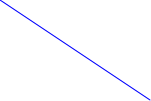
\includegraphics[scale=0.5]{videospiele/line1}|
(line -150 100 "blue")
|\evalsto| |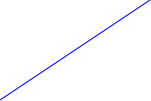
\includegraphics[scale=0.5]{videospiele/line2}|
\end{lstlisting}
%
Wir können auch ein Bild erzeugen, in dem Text steht, und zwar mit der
Funktion \lstinline{text}\indexvariable{text}, die folgende Signatur hat:
%
\begin{lstlisting}
(: text (string real color -> image))
\end{lstlisting}
%
Die Zahl ist die Höhe der Buchstaben.  Beispiel:
%
\begin{lstlisting}
(text "Schreibe Dein Programm!" 20 "red")
|\evalsto| |
\includegraphics[scale=0.5]{videospiele/text}|
\end{lstlisting}
%
Manchmal reichen einfache Rechtecke und Kreise nicht aus und wir
wollen komplexere Formen erzeugen.  Eine Möglichkeit ist die Funktion
\lstinline{polygon}\indexvariable{polygon}, die ein n-Eck
zeichnet.  Sie hat folgende Signatur:
%
\begin{lstlisting}
(: polygon ((list-of (mixed posn pulled-point)) mode color -> image)) 
\end{lstlisting}
%
Diese Funktion akzeptiert eine Liste von Eckpunkten und die üblichen
\lstinline{mode}- und \lstinline{color}"=Argumente.  Ein Eckpunkt 
muss entweder zur Signatur \lstinline{posn} oder zu
\lstinline{pulled-point} gehören.  Das sind eingebaute Record-Typen,
bei denen \lstinline{posn}\indexvariable{posn} so definiert sein könnte:
%
\indexvariable{posn}
\begin{lstlisting}
(define-record posn
  make-posn
  posn?
  (posn-x real)
  (posn-y real))
\end{lstlisting}
%
Dieser Typ definiert also ganz normale kartesische Koordinaten mit X-
und Y-Komponente.  Hier ist ein Beispiel für ein Polygon mit solchen
Eckpunkten:
%
\begin{lstlisting}
(polygon (list (make-posn 0 0)
               (make-posn -20 40)
               (make-posn 120 0)
               (make-posn -20 -40))
         "solid"
         "plum")
|\evalsto| |
\includegraphics[scale=0.5]{videospiele/polygon1}|
\end{lstlisting}
%
Bei \lstinline{posn}-Eckpunkten sind die Kanten also alles gerade
Linien.  Mit \lstinline{pulled-point}-Eckpunkten ist es möglich, die
Kanten zu Kurven zu machen.  Auch \lstinline{pulled-point} ist ein
Record-Typ:
%
\indexvariable{pulled-point}
\begin{lstlisting}
(define-record pulled-point
 make-pulled-point
 pulled-point?
 (pulled-point-lpull real)
 (pulled-point-langle real)
 (pulled-point-x real)
 (pulled-point-y real)
 (pulled-point-rpull real)
 (pulled-point-rangle real))
\end{lstlisting}
%
Wie \lstinline{posn} hat auch \lstinline{pulled-point} eine X- und
eine Y-Koordinate.  Außerdem gibt es jeweils zwei "<Pull">- und 
"<Angle">-Komponenten, die spezifizieren, wie die Kanten gebogen
werden.  Abbildung~\ref{fig:pulled-point} zeigt, wie das
funktioniert:  Für jeden Eckpunkt gibt es eine Kante vom
vorigen Punkt~-- die \emph{eingehende} Kante~-- und die Kante zum nächsten
Punkt~-- die \emph{ausgehende} Kante.

\begin{figure}[tb]
  \centering
  \def\svgwidth{0.4\textwidth}
  \input{videospiele/pulled-point.pdf_tex}
  \caption{Funktionsweise von \lstinline{pulled-point}}
  \label{fig:pulled-point}
\end{figure}
%
Die \lstinline{pulled-point-langle}-Komponente gibt den Winkel an, mit
dem die eingehende Kante gebogen wird, die
\lstinline{pulled-point-rangle}-Komponente den Winkel ist für die
ausgehende Kante zuständig.  Abbildung~\ref{fig:pulled-point} zeigt,
in welche Richtung \lstinline{langle} und \lstinline{rangle} die
beiden Kanten von Punkt Nummer~2 biegen: Die eingehende Kante kommt von Punkt~1 her, die
ausgehende Kante geht zu Punkt~3.  Die Komponenten
\lstinline{pulled-point-lpull} und \lstinline{pulled-point-rpull}
geben an, wieviel die Kanten verbogen werden auf einer Skala zwischen $0$ und $1$.
%
\begin{lstlisting}
(polygon (list (make-pulled-point 1/2 0 0 0 1/2 -20)
               (make-posn -20 40)
               (make-pulled-point 1/2 -20 120 0 1/2 20)
               (make-posn -20 -40))
         "solid"
         "plum")
|\evalsto| |
\includegraphics[scale=0.5]{videospiele/polygon2}|
\end{lstlisting}
%
\begin{figure}[tb]
  \centering
  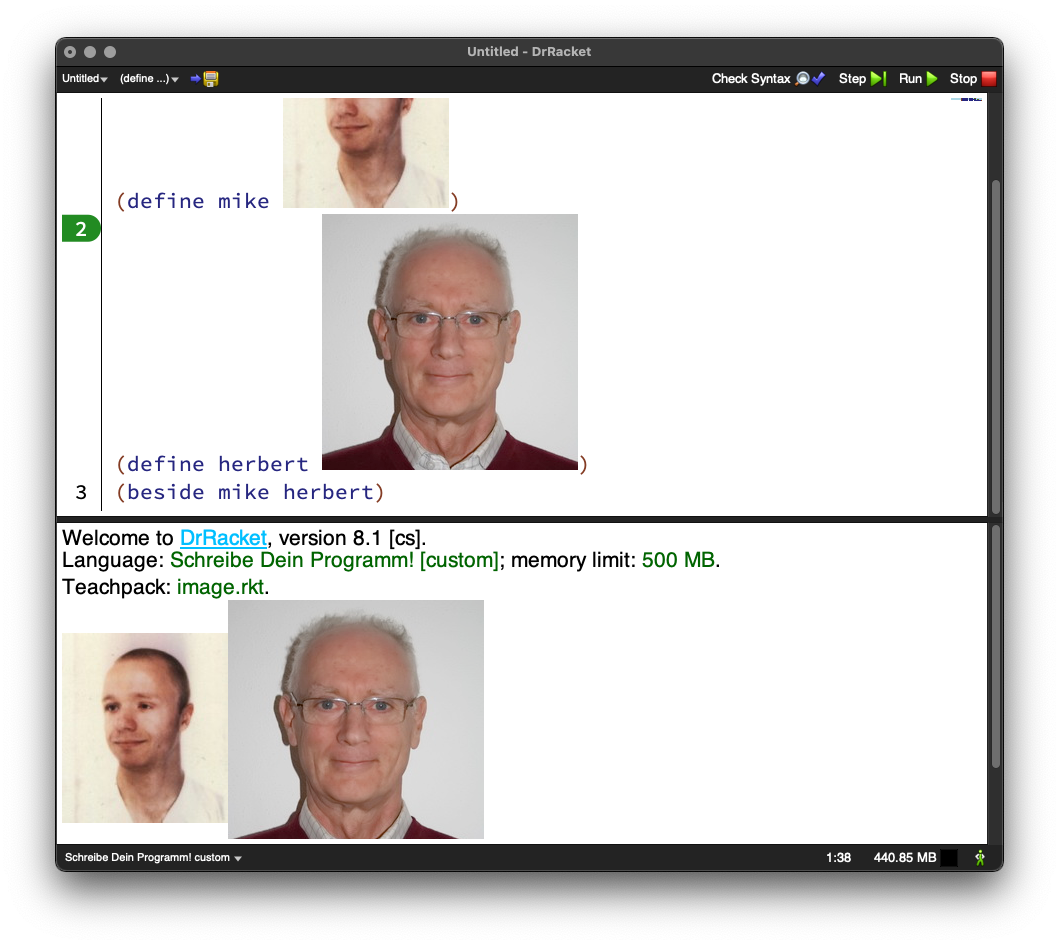
\includegraphics[height=0.4\textheight]{videospiele/insert-image}
  \caption{Bilddatei in Programm einbetten}
  \label{fig:image-insert}
\end{figure}
Es ist auch möglich, Bilder-Dateien in
\texttt{image.rkt}-Bilder zu verwandeln.  Das macht der Menüpunkt
\texttt{Bild einfügen} im \texttt{Spezial}-Menü.
Alternativ ist es möglich,
Bilder in anderen Applikationen auszuwählen und zu kopieren und dann
in DrRacket einzufügen.  Die eingefügten Bilder dienen dann als
Literale für Bild-Werte.  Abbildung~\ref{fig:image-insert} zeigt ein
Beispiel.

Schließlich ermitteln die folgenden Funktionen Breite und Höhe
eines Bildes:\indexvariable{image-width}\indexvariable{image-height}
%
\begin{lstlisting}
(: image-width  (image -> natural))
(: image-height (image -> natural))
\end{lstlisting}
%

\subsection{Bilder zusammensetzen und verändern}

Da diese geometrischen Formen für sich genommen langweilig sind,
können wir mehrere Bilder zu einem zusammensetzen.

Zum Aufeinanderlegen gibt es die Funktion
\lstinline{overlay}\indexvariable{overlay}, die ein Bild
mittig auf ein anderes Bild drauflegt.  Das Ergebnis
ist groß genug, dass beide
Bilder hineinpassen.  Signatur und Beispiel:
%
\begin{lstlisting}
(: overlay (image image -> image))

(overlay
  (circle 50 "solid" "gold")
  (rectangle 100 100 "solid" "blue"))
|\evalsto| |
\includegraphics[scale=0.5]{videospiele/overlay}|
\end{lstlisting}
%
Die
Funktion~\lstinline{overlay/xy}\indexvariable{overlayxy}
erlaubt, das untere Bild gegenüber dem oberen in X- und Y-Richtung zu
verschieben.  Signatur und Beispiel:%
\begin{lstlisting}
(: overlay/xy (image real real image -> image))

(overlay/xy
  (circle 50 "solid" "gold")
  10 -20
  (rectangle 100 100 "solid" "blue"))
|\evalsto| |
\includegraphics[scale=0.5]{videospiele/overlayxy}|
\end{lstlisting}
%
Das Beispiel zeigt, das auch \lstinline{overlay/xy} das Ergebnisbild
gerade so groß macht, dass die beiden Eingabebilder hineinpassen.

Manchmal macht auch \lstinline{overlay/xy} nicht das richtige, nämlich
wenn einfach nur ein Bild in eine "<Szene"> platziert werden soll,
zum Beispiel das Gürteltier auf einem Straßenabschnitt.  In dem Fall
wollen wir genau wie bei \lstinline{overlay/xy} kontrollieren, an
welchen Koordinaten das daraufgelegte Bild erscheint, aber das Bild
soll nicht größer werden, wenn zum Beispiel ein Teil des Gürteltiers
über den Straßenabschnitt hinausragt.  Diese Aufgabe erledigt die
Funktion
\lstinline{place-iamge}\indexvariable{place-image}, deren
Signatur der von \lstinline{overlay/xy} entspricht:
%
\begin{lstlisting}
(: place-image (image real real image -> image))
\end{lstlisting}
%
Die beiden Koordinaten werden anders als bei
\lstinline{overlay/xy} nicht relativ zur mittigen Anordnung
interpretiert.  Stattdessen geben die beiden Koordinaten die Position
im zweiten Bild an, wo die Mitte des ersten Bilds platziert wird,
ausgehend von der oberen linken Ecke des ersten Bildes:
%
\begin{lstlisting}
(place-image
  (circle 50 "solid" "gold")
  40 70
  (rectangle 100 100 "solid" "blue"))
|\evalsto| |
\includegraphics[scale=0.5]{videospiele/place-image}|
\end{lstlisting}
%
Die Funktion \lstinline{place-image} hat noch eine große Schwester
\lstinline{place-image/align}.\indexvariable{place-image-align}\label{func:place-image-align}
Während \lstinline{place-image} den Bezugspunkt in der Mitte des
ersten Bilds setzt, erlaubt \lstinline{place-image} auch anderee
Bezugspunkte.
Hier die Signatur:
%
\begin{lstlisting}
(: place-image/align (image real real x-place y-place image -> image))
\end{lstlisting}
%
Die Signaturen \lstinline{x-place} und \lstinline{y-place} könnten
folgendermaßen definiert sein:
%
\indexvariable{x-place}
\indexvariable{y-place}
\begin{lstlisting}
(define x-place (signature (enum "left" "right" "center")))
(define y-place (signature (enum "top" "bottom" "center")))
\end{lstlisting}
%
Diese Argumente geben an, ob der Bezugspunkt horizontal am linken
oder rechten Rand oder in der Mitte liegt und vertikal oben, unten
oder in der Mitte:
%
\begin{lstlisting}
(place-image/align
  (circle 20 "solid" "gold")
  40 70 "left" "center"
  (rectangle 100 100 "solid" "blue"))
|\evalsto| |
\includegraphics[scale=0.5]{videospiele/place-image-align1}|

(place-image/align
  (circle 20 "solid" "gold")
  40 70 "right" "center"
  (rectangle 100 100 "solid" "blue"))
|\evalsto| |
\includegraphics[scale=0.5]{videospiele/place-image-align2}|

(place-image/align
  (circle 20 "solid" "gold")
  40 70 "center" "center"
  (rectangle 100 100 "solid" "blue"))
|\evalsto| |
\includegraphics[scale=0.5]{videospiele/place-image-align3}|

(place-image/align
  (circle 20 "solid" "gold")
  40 70 "center" "top"
  (rectangle 100 100 "solid" "blue"))
|\evalsto| |
\includegraphics[scale=0.5]{videospiele/place-image-align4}|

(place-image/align
  (circle 20 "solid" "gold")
  40 70 "center" "bottom"
  (rectangle 100 100 "solid" "blue"))
|\evalsto| |
\includegraphics[scale=0.5]{videospiele/place-image-align5}|
\end{lstlisting}
%
Die folgenden Funktionen \lstinline{above} und \lstinline{beside}
kennst Du vielleicht noch aus dem ersten Kapitel auf
Seite~\pageref{function:beside-above}.  Sie setzten zwei Bilder
übereinander respektive nebeneinander:
% 
\begin{lstlisting}
(: above  (image image -> image))
(: beside (image image -> image))
\end{lstlisting}
%
Manchmal sieht ein Bild gut aus, ist aber zu klein oder zu groß
geraten.  Die Funktion \lstinline{scale} kann es größer oder kleiner
machen.  Signatur:
\begin{lstlisting}
(: scale (real image -> image))
\end{lstlisting}
%
Beispiel:
%
\begin{lstlisting}
(define c (circle 20 "solid" "green"))
(beside (scale 0.5 c)
        c
        (scale 1 c)
        (scale 1.5 c)
        (scale 2 c)
        (scale 3 c))
|\evalsto| |
\includegraphics[scale=0.5]{videospiele/scale}|
\end{lstlisting}

\section{Modelle und Ansichten}

\mentioncode{videospiele/dillo-world.rkt}
%
In unserem Videospiel geht es um Gürteltiere auf dem texanischen
Highway.  Vielleicht erinnerst Du Dich, wir sind ihnen schon in
Abschnitt~\ref{sec:armadillo} auf Seite~\pageref{sec:armadillo}
begegnet:
%
\indexvariable{run-over-dillo}
\indexvariable{dillo}
\begin{lstlisting}
; Ein Gürteltier hat folgende Eigenschaften:
; - Gewicht (in g)
; - lebendig oder tot
(define-record dillo
  make-dillo
  dillo?
  (dillo-weight natural)
  (dillo-alive? boolean))

(: make-dillo (natural boolean -> dillo))
(: dillo-weight (dillo -> natural))
(: dillo-alive? (dillo -> boolean))

(define dillo1 (make-dillo 55000 #t)) ; 55 kg, lebendig 
(define dillo2 (make-dillo 58000 #f)) ; 58 kg, tot
(define dillo3 (make-dillo 60000 #t)) ; 60 kg, lebendig
(define dillo4 (make-dillo 63000 #f)) ; 63 kg, tot

; Gürteltier überfahren
(: run-over-dillo (dillo -> dillo))

(define run-over-dillo
  (lambda (dillo)
    (make-dillo (dillo-weight dillo)
                #f)))
\end{lstlisting}
%
Die Datendefinition mit dem zugehörigen Code hält zwar einige Eigenschaften
von Gürteltieren fest, für ein Videospiel fehlt aber eine
grafische Darstellung.  Eine solche Repräsentation mit
zugehörigen Operationen heißt in der Softwararchitektur auch
\textit{Modell}\index{Modell} oder auch
\textit{Domänenlogik}\index{Domänenlogik}, und bei größeren Softwaresystemen
ist es eine gute Idee, das Modell von der grafischen Darstellung zu
trennen, damit das Modell stabil bleiben kann, auch wenn die grafische
Darstellung geändert wird.

Die grafische Darstellung eines Modells nennen wir dessen
\textit{Ansicht}\index{Ansicht} (auf englisch
\textit{View}\index{View}).  Wenn wir uns also mit Gürteltieren als
Modell für ein Videospiel beschäftigen, müssen wir daraus eine Ansicht
in Form eines Bildes berechnen.

Wir warnen Dich schonmal vor: Der grafische Gestaltung in diesem
Kapitel fehlt es an Finesse.  Wir hoffen, Du kannst
sie verbessern!

Die folgende Funktion macht aus einem \lstinline{dillo}-Wert ein Bild:
%
\begin{lstlisting}
; Gürteltier-Bild erzeugen
(: dillo-image (dillo -> image))
\end{lstlisting}
%
\begin{figure}[tb]
  \centering
  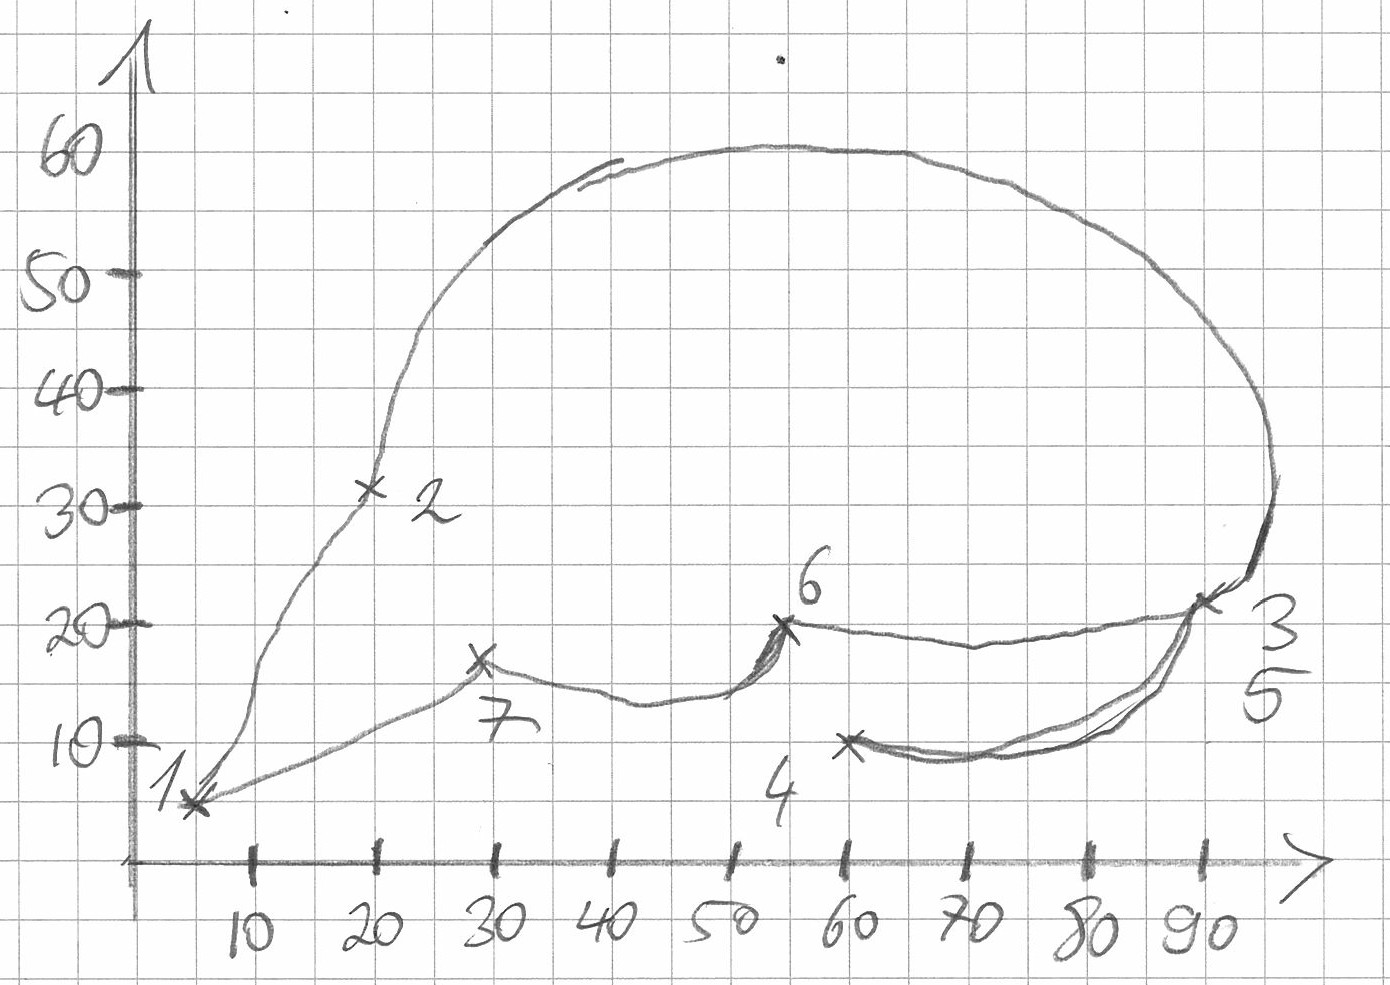
\includegraphics[width=0.6\textwidth]{videospiele/dillo}
  \caption{Umriss eines Gürteltiers}
  \label{fig:dillo-body}
\end{figure}
Als Basis dafür machen wir erstmal ein Bild mit dem Körper des
Gürteltiers.  Zu diesem Zweck haben wir in
Abbildung~\ref{fig:dillo-body} zunächst von Hand eine
Zeichnung mit dem Umriss des Gürteltiers in ein Koordinatensystem
gezeichnet und die Punkte markiert, an denen sich die Richtung des
Strichs abrupt ändert~-- also quasi die Ecken.  Diese Ecken haben wir
durchnummeriert und daraus haben wir dieses Polygon gemacht:
%
\indexvariable{dillo-body}
\begin{lstlisting}
(define dillo-body
  (overlay/xy (polygon
               (list (make-pulled-point 0.3 30
                                        5 (- 60 5)
                                        0.2 5)
                     (make-pulled-point 0.4 20
                                        20 (- 60 32)
                                        0.5 -70)
                     (make-pulled-point 0.5 120 
                                        90 (- 60 22)
                                        0.2 -30)
                     (make-pulled-point 0.5 90
                                        60 (- 60 10)
                                        0.5 90)
                     (make-pulled-point 0 0 
                                        90 (- 60 22)
                                        0.2 -30)
                     (make-pulled-point 0 0
                                        55 (- 60 20)
                                        0.3 -30)
                     (make-pulled-point 0 0
                                        29 (- 60 17)
                                        0.5 20))
               "solid"
               "brown")
              0 -30
              (rectangle 100 60
                         "solid" "transparent")))
\end{lstlisting}
%
Du siehst, da haben wir ganz schön viel herumprobiert, bis es
einigermaßen aussah, insbesondere bei den Zahlen für die
\lstinline{pulled-point}s.  Immerhin haben wir die Koordinaten aus der
Zeichnung direkt übertragen, dabei ist uns aber aufgefallen, dass die
Koordinaten in der Mathematik von unten nach oben, im Teachpack aber
von oben nach unten laufen.  Darum steht da zum Beispiel
\lstinline{(- 60 5)} für die Y-Koordinate 5, weil der obere Rand der
Zeichnung bei 60 liegt.

Außerdem ist das Gürteltier vor allem nach oben und rechts nach außen
gewölbt.  DrRacket schneidet das Polygon bei der Anzeige ab, weswegen
wir es mit \lstinline{overlay/xy} noch auf einen transparenten
Hintergrund montiert haben.  So sieht das Ergebnis aus:
%
\begin{lstlisting}
dillo-body
|\evalsto| |
\includegraphics[scale=0.5]{videospiele/dillo-body}|
\end{lstlisting}
%
Jetzt wollen wir ja nicht jedes Gürteltier genau gleich darstellen,
sondern wir wollen dessen Eigenschaften bei der Darstellung
berücksichtigen.  Dafür schreiben wir die Funktion
\lstinline{dillo-image}, von der wir ja schon Kurzbeschreibung und
Signatur gesehen haben.  Hier ist das Gerüst mit der Schablone für
zusammengesetzte Daten als Eingabe:
%
\begin{lstlisting}
(define dillo-image
  (lambda (dillo)
    ... 
    (dillo-weight dillo)
    (dillo-alive? dillo)
    ...))
\end{lstlisting}
%
Wir sollten also noch berücksichtigen, wieviel das Gürteltier wiegt
und außerdem, ob es noch lebt.  Das Gewicht berücksichtigen wir, indem
wir das Gürteltier größer oder kleiner machen:
%
\begin{lstlisting}
(define dillo-image
  (lambda (dillo)
    (scale (+ 1
              (/ (- (dillo-weight dillo) 50000)
                 15000))
           dillo-body)
    ...
    (dillo-alive? dillo)
    ...))    
\end{lstlisting}
%
Den Faktor bei \lstinline{scale} haben wir durch Probieren
ermittelt.  Aber \lstinline{(dillo-alive? dillo)} steht noch da~-- wir
bauen das ein, indem wir einem toten Gürteltier "<tote Augen"> ins
Gesicht setzen:
%
\indexvariable{dillo-image}
\indexvariable{dead-eyes}
\begin{lstlisting}
(define dillo-image
  (lambda (dillo)
    (scale (+ 1
              (/ (- (dillo-weight dillo) 50000)
                 15000))
           (if (dillo-alive? dillo)
               dillo-body
               (overlay/xy dead-eyes
                           -25 -25
                           dillo-body)))))

(define dead-eyes
  (overlay (line 10 10 "green")
           (line -10 10 "green")))
\end{lstlisting}
%
\section{Den Highway modellieren}
\label{sec:highway-model}

\begin{figure}[tb]
  \centering
  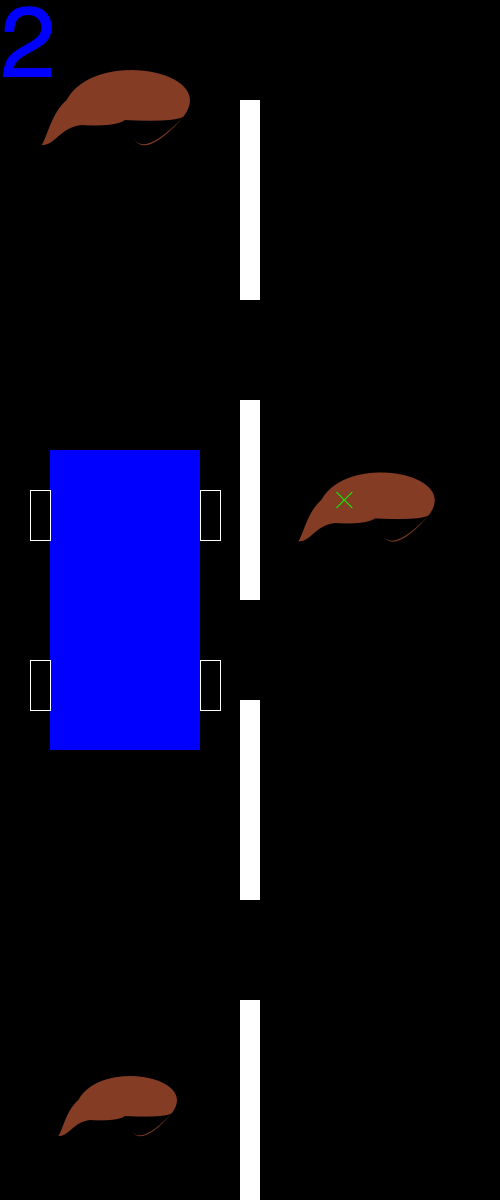
\includegraphics[height=0.4\textheight]{videospiele/dillo-world}
  \caption{Gürteltiere auf der Straße}
  \label{fig:dillo-world}
\end{figure}

Ein Gürteltier allein macht noch kein Videospiel: Wir setzen gleich
mehrere Gürteltiere auf die Straße und~-- natürlich~-- überfahren sie
dann.  Das sieht dann so aus wie in
Abbildung~\ref{fig:dillo-world}. Das Auto bewegt sich auf der Straße
und kann entweder auf die linke oder rechte Straßenseite wechseln, wo
es dann gegebenfalls über Gürteltiere fährt.  Oben links steht ein
Punktestand~-- wieviele Gürteltiere schon vom lebenden Zustand in den
toten überführt wurden.

Damit wir das alles darstellen können, müssen für alles
Datendefinition schreiben, was auf dem Bild der Straße zu sehen sind:
%
\begin{itemize}
\item die Position des Autos
\item die Positionen der Gürteltiere zusammen mit ihren Zuständen
\item der Punktestand
\end{itemize}
%
Für diese Aspekte des Spiels entwickeln wir Datendefinitionen.
Man sieht schon, dass "<Positionen"> eine wichtige Rolle spielen,
sowohl für das Auto als auch für die Gürteltiere.  In dem Bild kann
man sehen, dass dazu gehört, auf welcher Seite der Straße sich etwas
aufhält und bei welchem "<Straßenmeter">.  
Hier sind Datendefinitionen für die Straßenseite und die Position heraus:
%
\indexvariable{side}
\indexvariable{position}
\begin{lstlisting}
; Straßenseite
(define side
  (signature (enum "left" "right")))

; Eine Position auf der Straße besteht aus:
; - Straßenmeter (Abstand vom Straßenanfang in Meter)
; - Seite
(define-record position
  make-position
  position?
  (position-m-from-start real)
  (position-side side))
\end{lstlisting}
%
Als nächstes müssen wir die Idee "<Positionen der Gürteltiere zusammen
mit ihren Zuständen"> in eine Datendefinition umwandeln.  Wir machen
das erstmal für ein einzelnes Gürteltier und nennen das Konzept
"<Gürteltier auf der Straße">:
%
\indexvariable{dillo-on-road}
\begin{lstlisting}
; Ein Gürteltier auf der Straße hat folgende Eigenschaften:
; - Gürteltier-Zustand
; - Position auf der Straße
(define-record dillo-on-road
  make-dillo-on-road
  dillo-on-road?
  (dillo-on-road-state dillo)
  (dillo-on-road-position position))
\end{lstlisting}
%

\section{Straßenansichten}

Jetzt wo wir die Welt modelliert haben können wir sie auch auf den
Bildschirm bringen.  Wir fangen erstmal mit den einfachen und
offensichtlichen Elementen an: der Straße, inklusive der
Markierung auf dem Mittelstreifen und dem Auto.  Die Gürteltiere
haben wir ja schon.

Damit wir einigermaßen realistisch über die Proportionen von allem
nachdenken können, messen wir alles in Metern ab und wandeln zwischen
Metern und Pixeln hin und her.  Auf unserem Bildschirm sieht ein
Verhältnis von 1m:100 Pixel gut aus.  Diese Funktionen konvertieren
hin und her:

\indexvariable{meters->pixels}
\indexvariable{pixels->meters}
\begin{lstlisting}
; Meter in Pixel umwandeln
(: meters->pixels (real -> real))

(define meters->pixels
  (lambda (meters)
    (* meters 100)))

; Pixel in Meter umwandeln
(: pixels->meters (real -> real))

(define pixels->meters
  (lambda (pixels)
    (/ pixels 100)))
\end{lstlisting}
%
Die Straße selbst ist nur ein schwarzes Rechteck, das ist einfach.
Schwieriger sind die Straßenmarkierungen, also abwechselnd ein weißer
und ein schwarzer Streifen.  Damit das realistisch aussieht,
definieeren wir erst einmal die Länge der Markierungen und die der Lücken:
%
\indexvariable{marking-height}
\indexvariable{gap-height}
\begin{lstlisting}
(define marking-height 2) ; Höhe der Streifen
(define gap-height 1) ; Höhe der Lücken
\end{lstlisting}
%
Die Markierungen und die Lücken müssen wir abwechseln
aneinanderkleben.  Wie oft fragst Du?  Nun, der texanische Highway ist
unendlich lang, das wäre schwierig.  Aber wir zeigen ja nur einen
Ausschnitt, und darum machen wir nur soviele Streifen, wie in den
Ausschnitt passen.  Wieviele das sind, hängt von der Höhe des
Ausschnitts ab.  Wir könnten natürlich von Hand nachzählen, das würde
aber bedeuten, dass wir uns frühzeitig auf die Höhe des Ausschnitts
festlegen müssten.  Um das zu vermeiden, schreiben wir erst einmal
eine Funktion, die als Eingabe die Anzahl der Streifen akzeptiert.
Wir folgen der Schablone für Funktionen auf natürlichen Zahlen:
%
\indexvariable{markings}
\begin{lstlisting}
; Straßenmarkierung mit bestimmter Anzahl von Streifen malen
(: markings (natural -> image))

(define markings
  (lambda (n)
    (cond
      ((zero? n) empty-image)
      ((positive? n)
       (above (rectangle (meters->pixels .20)
                         (meters->pixels marking-height)
                         "solid"
                         "white")
              (rectangle (meters->pixels .20)
                         (meters->pixels gap-height)
                         "solid"
                         "black")
              (markings (- n 1)))))))
\end{lstlisting}
%
Hier jetzt die tatsächliche Höhe des Straßenabschnitts:
%
\indexvariable{road-window-height}
\begin{lstlisting}
(define road-window-height 12) ; Höhe des Straßenausschnitts
\end{lstlisting}
%
Die Idee ist, dass Du später nur diese eine Definition ändern musst, falls
Dir die Ausschnittshöhe nicht passt, und sich dann alles andere
automatisch anpasst.

Um die Anzahl der nötigen Markierungen zu berechnen, teilen wir die
Höhe des Straßenausschnitts durch die Länge einer Markierung plus
Lücke.  Zur Sicherheit addieren wir noch eins drauf: Die Division könnte
nicht ganz aufgehen.  Außerdem wird möglicherweise am Ende nur ein
Teil eines Streifens zu sehen sein, auch dafür ist es gut, wenn im
Zweifelsfall einer mehr da ist.
%
\indexvariable{marking-count}
\begin{lstlisting}
; Anzahl der nötigen Markierungen
(define marking-count
  (+ 1
     (quotient road-window-height
               (+ marking-height gap-height))))
\end{lstlisting}
%
Aus der Zahl machen wir schließlich
das Bild der Streifen:
%
\indexvariable{visible-markings}
\begin{lstlisting}
; sichtbare Markierungen
(define visible-markings
  (markings marking-count))
\end{lstlisting}
%
Zur Erinnerung: Die Funktion \lstinline{quotient} haben wir auf
Seite~\pageref{func:quotient} eingeführt, sie teilt ganzzahlig.

Nun können wir das Bild des Straßenausschnitts zusammensetzen.  Wir
brauchen neben der Höhe auch noch die Breite und machen erstmal eine
leere Szene nur aus schwarzem Asphalt:
%
\indexvariable{road-width}
\indexvariable{blank-road-window}
\begin{lstlisting}
; in Meter
(define road-width 5)

(define blank-road-window
  (empty-scene (meters->pixels road-width)
               (meters->pixels road-window-height)
               "black"))
\end{lstlisting}
%
Wie Mittelstreifen auf dem Straßenausschnitt platziert werden, hängt
davon ab, an welchem Straßenmeter sich der Bildausschnitt befindet.
Wir schreiben also eine Funktion, welche die Straßenmeter akzeptiert
und ein passendes Bild liefert:
\begin{lstlisting}
; Straßenausschnitt anzeigen
(: road-window (real -> image))
\end{lstlisting}
%
Wir benutzen \lstinline{place-image/align} (siehe
Seite~\pageref{func:place-image-align}), um die Mittelstreifen auf den
Asphalt zu setzen:
%
\begin{lstlisting}
(define road-window
  (lambda (meters)
    (place-image/align visible-markings
                       ...
                       ...
                       ... ...
                       blank-road-window)))
\end{lstlisting}
%
Wir setzen zunächst den Bezugspunkt beim Mittelstreifen nach oben in
die Mitte:
%
\begin{lstlisting}
(define road-window
  (lambda (meters)
    (place-image/align visible-markings
                       ...
                       ...
                       "center" "top"
                       blank-road-window)))
\end{lstlisting}
%
In X-Richtung muss der Mittelstreifen in die Mitte, da können wir
einfach die Breite der Straße halbieren.

Bei der Y-Koordinate ist es schwieriger: Die hängt von den
Straßenmetern ab.  Die Straßenmeter sind aber (außer ganz am Anfang)
mehr als der Ausschnitt hoch beziehungsweise das Mittelstreifenbild
lang ist.  Das Mittelstreifenbild wiederholt sich aber immer, wenn ein
Streifen plus Lücke vorbeigezogen ist.  Wir rechnen also die Anzahl
der Pixel dafür aus:
%
\indexvariable{marking-segment-pixels}
\begin{lstlisting}
(define marking-segment-pixels
  (meters->pixels (+ marking-height gap-height)))
\end{lstlisting}
%
Durch diese Zahl teilen wir und nehmen den Divisionsrest, um die
Y-Position zu bekommen.  Das heißt nicht ganz~-- der Divisionsrest ist immer
positiv, und damit ist der Mittelstreifen zu weit unten: Wir ziehen
das Bild noch um einen Streifen nach oben, indem wir
\lstinline{marking-segment-pixels} abziehen.  Das kommt dabei heraus:
%
\indexvariable{road-window}
\begin{lstlisting}
(define road-window
  (lambda (meters)
    (place-image/align visible-markings
                       (/ (image-width blank-road-window) 2)
                       (- (remainder (meters->pixels meters)
                                     marking-segment-pixels)
                          marking-segment-pixels)
                       "center" "top"
                       blank-road-window)))
\end{lstlisting}
%
\begin{aufgabeinline}
  Probiere \lstinline{road-window} aus.  Entferne die Substraktion von
  \lstinline{marking-segment-pixels} und untersucht, wie sich das
  auswirkt!
\end{aufgabeinline}
%

\section{Bewegte Bilder mit \texttt{universe.rkt}}

Bisher haben wir nur statische, langweilige Bilder.  Es ist Zeit, sie
in Bewegung zu setzen.  Dafür brauchen wir ein weiteres Teachpack
namens \texttt{universe.rkt}.  Um es zu aktivieren, musst Du nochmal
ins \texttt{Sprache}/\texttt{Language}-Menü und dort auf
\texttt{Teachpack hinzufügen}/\texttt{Add Teachpack} drücken und in
dem dann auftauchenden Dialog auf \texttt{universe.rkt} und
schließlich auf \texttt{OK} drücken.

Zum \texttt{universe.rkt}-Teachpack gehört eine Funktion namens
\lstinline{animate}\indexvariable{animate}.  Was sie macht,
verdeutlicht am einfachsten ein Beispiel, dass Du in die REPL
eintippen kannst:
%
\begin{lstlisting}
(animate
  (lambda (ticks)
     (place-image/align (circle 5 "solid" "red") 
                        100 ticks "center" "top" 
                        (square 200 "solid" "black"))))
\end{lstlisting}
%
\begin{aufgabeinline}
  Probier es aus!
\end{aufgabeinline}
%
Du siehst einen kleinen roten Kreis sich in einem quadratischen Bild
von oben nach unten bewegen. 

Die neue Funktion \lstinline{animate} akzeptiert eine Funktion mit
einer Eingabe names \lstinline{ticks}, die ein Bild produziert:
%
\begin{lstlisting}
(: animate ((natural -> image) -> natural))
\end{lstlisting}
%
\lstinline{Animate} ruft die Funktion 28mal in der Sekunde auf und
zeigt die entstehenden Bilder hintereinander als Animation an.  Dabei
übergibt \lstinline{animate} als \lstinline{ticks} eine natürliche
Zahl, die bei Null anfängt, und jedesmal um eins größer wird: Sie
misst also die Zeit, in sogenannten \textit{Ticks}\index{Ticks}.

Wir benutzen jetzt \lstinline{animate}, um das Bild des
Straßenausschnitts in Bewegung zu setzen~-- so, dass das Wagen genau
in der Mitte ist.  Wir legen zuerst fest, wie schnell der Wagen fährt.
Wir haben uns für ein recht gemächliches Tempo entschieden, damit wir auch
wirklich alle Gürteltiere erwischen:
%
\indexvariable{meters-per-tick}
\begin{lstlisting}
; Meter pro Tick
(define meters-per-tick 0.1)
\end{lstlisting}
%
Diese Funktion ist so einfach, dass sich ausnahmsweise separates
Testen nicht lohnt:
%
\indexvariable{ticks->meters}
\begin{lstlisting}
; Ticks in Meter umwandeln
(: ticks->meters (natural -> rational))

(define ticks->meters
  (lambda (ticks)
    (* meters-per-tick ticks)))
\end{lstlisting}
%
Damit schreiben wir Funktion, die aus Ticks Straßenmeter
macht und \lstinline{road-window} aufruft:
%
\indexvariable{road-window-at-ticks}
\begin{lstlisting}
; Straßenausschnitt zu Zeitpunkt anzeigen
(: road-window-at-ticks (natural -> image))

(define road-window-at-ticks
  (lambda (ticks)
    (road-window (ticks->meters ticks))))
\end{lstlisting}
% Du kannst
also folgendes ausprobieren:
%
\begin{lstlisting}
(animate road-window-at-ticks)
\end{lstlisting}
%
\begin{aufgabeinline}
  Schreibe eine andere Funktion Deiner Wahl mit der für
  \lstinline{animate} passenden Signatur und probiere
  \lstinline{animate} damit aus!
\end{aufgabeinline}

\section{Autos und Gürteltiere auf dem Highway}

Die Straße ist fertig, als nächstes ist das Auto dran.  Wir fangen mit
einem Rad an:
%
\indexvariable{wheel}
\begin{lstlisting}
; Rad
(define wheel
  (rectangle (meters->pixels 0.2) (meters->pixels .5)
             "outline" "white"))
\end{lstlisting}
%
Als nächstes setzen wir zwei Räder zu einem Bild zusammen, das dann
links und rechts von der Karosserie platziert werden:
%
\indexvariable{wheels-on-one-side}
\indexvariable{car-width}
\indexvariable{car-length}
\indexvariable{car}
\begin{lstlisting}
; Zwei Räder auf einer Seite des Autos
(define wheels-on-one-side
  (above wheel
         (rectangle 0 (meters->pixels 1.2) "solid" "black")
         wheel))

; Breite des Autos
(define car-width 1.5)
; Länge des Autos
(define car-length 3.0)
 
; Bild des Autos
(define car
  (beside
   wheels-on-one-side
   (rectangle (meters->pixels car-width) (meters->pixels car-length)
              "solid" "blue")
   wheels-on-one-side))
\end{lstlisting}
%
Schließlich müssen wir Auto und Gürteltiere auf der
Straße platzieren.  Bei der Funktion dafür ist klar, dass ein Bild
herauskommen soll.  Als Eingaben stehen schon einmal fest:
%
\begin{itemize}
\item das Bild, das auf der Straße platziert werden soll
\item die Position des Bildes
\end{itemize}
%
Wir benötigen außerdem noch:
%
\begin{itemize}
\item die Zeit, weil sie bestimmt, welcher Ausschnitt der Straße
  angezeigt wird
\item das Bild der Straße
\end{itemize}
%
Letzteres überrascht Dich vielleicht. Ist das Bild der Straße nicht
immer das gleiche?  Nein, ist es nicht!  Zunächst einmal ist die
Position des Mittelstreifens je nach Zeit immer unterschiedlich.
Außerdem wollen wir ja nicht nur ein Bild auf der Straße platzieren,
sondern viele.  Dafür füttern wir das Ergebnis der Funktion wieder in
die Funktion hinein, um ein weiteres Bild zu platzieren.

Kurzbeschreibung, Signatur und Gerüst sehen entsprechend aus wie
folgt:
%
\begin{lstlisting}
; Bild auf der Straße platzieren
(: place-image-on-road (image natural image position -> image))

(define place-image-on-road
  (lambda (road-image ticks image position)
    ...))
\end{lstlisting}
%
Da es sich bei \lstinline{position} um zusammengesetzte Daten handelt,
stehen in der Schablone Aufrufe der Selektoren:
%
\begin{lstlisting}
(define place-image-on-road
  (lambda (road-image ticks image position)
    ...
    (position-m-from-start position)
    (position-side position)
    ...))
\end{lstlisting}
%
Wir müssen jetzt die Pixelkoordinaten des Bildes relativ zum
Straßenausschnitt berechnen.  Bei der X-Koordinate ist das
verhältnismäßig einfach.  Wir legen eine Variable 
\lstinline{pixels-from-left} an, die sich aus 
\lstinline{(position-side position))} ergibt, 
was schon in der Schablone steht.  Die Seite
ist relativ zum Mittelstreifen, für dessen X-Koordinate wir ebenfalls
eine Zwischenvariable anlegen:
%
\begin{lstlisting}
    ; X-Koordinate der Mitte der Straße, in Pixeln
    (define middle-pixels (/ (image-width road-image) 2))
\end{lstlisting}
%
Daraus ergibt sich \lstinline{pixels-from-left} so:
%
\begin{lstlisting}
    ; X-Koordinate des Mittelpunkts des Bilds
    (define pixels-from-left
      (cond
        ((string=? (position-side position) "left")
         (* middle-pixels 0.5)) ; Mitte der linken Spur
        ((string=? (position-side position) "right")
         (* middle-pixels 1.5)))) ; Mitte der rechten Spur
\end{lstlisting}
%
Als nächstes brauchen wir die Y-Koordinate, da ist es etwas
komplizierter: Wir benötigen die Y-Koordinate von \lstinline{image}
\emph{relativ} zum unteren Rand des Bildes.  (Oder des oberen, das
geht auch.)  Das wäre folgender Ausdruck:
%
\begin{lstlisting}
(- (position-m-from-start position)
   (ticks->meters ticks))
\end{lstlisting}
%
Diese Koordinate ist noch in Metern, die müssen wir noch in Pixel
umrechnen.  Außerdem müssen wir berücksichtigen, dass die
Pixel-Koordinaten von oben nach unten laufen, die Straßenmeter aber
von unten nach oben~-- wir ziehen also diese Zahl von der Höhe des
Bildes ab.  Damit können wir wieder einmal
\lstinline{place-image/align} (siehe
Seite~\pageref{func:place-image-align}) bemühen, um das Bild auf die
Straße zu setzen.  Die Funktion sieht vollständig so aus:
%
\indexvariable{place-image-on-road}
\begin{lstlisting}
(define place-image-on-road
  (lambda (road-image ticks image position)
    ; X-Koordinate der Mitte der Straße, in Pixeln
    (define middle-pixels (/ (image-width road-image) 2))

    ; X-Koordinate des Mittelpunkts des Bilds
    (define pixels-from-left
      (cond
        ((string=? (position-side position) "left")
         (* middle-pixels 0.5)) ; Mitte der linken Spur
        ((string=? (position-side position) "right")
         (* middle-pixels 1.5)))) ; Mitte der rechten Spur

    (place-image/align
     image
     pixels-from-left
     (- (image-height road-image)
        (meters->pixels (- (position-m-from-start position)
                           (ticks->meters ticks))))
     "center" "center"
     road-image)))
\end{lstlisting}
%
Die Funktion ist kompliziert genug, dass wir sie testen sollten.
Einen \lstinline{check-expect}-Test vorab zu konstruieren ist schier
unmöglich, aber wir können die Funktion zumindest in der REPL
ausprobieren, am einfachsten bei $0$ Ticks, also am Anfang des Spiels:
%
\begin{lstlisting}
(place-image-on-road (road-window 0) 0 car (make-position 0 "left"))
|\evalsto{} 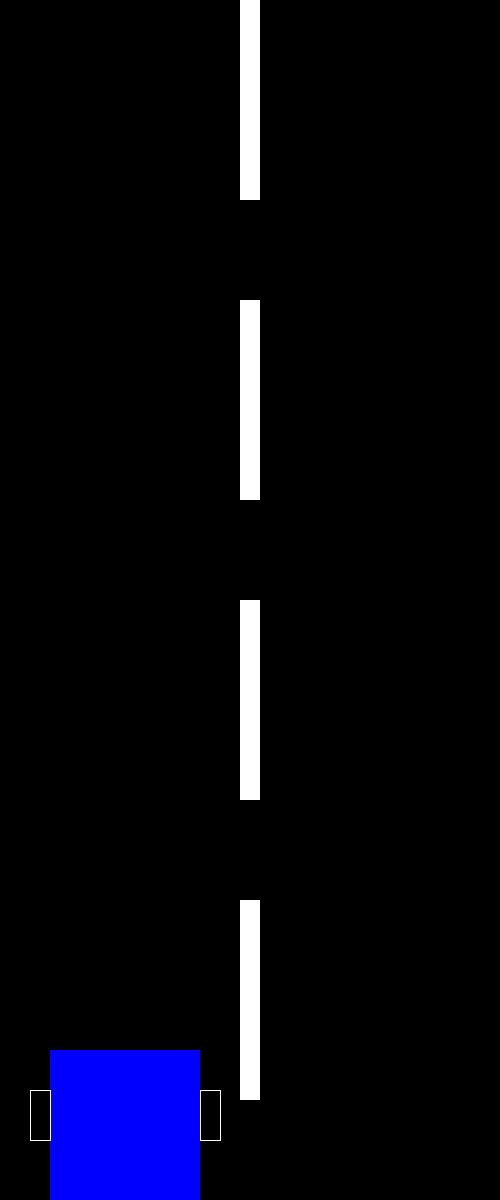
\includegraphics[height=1.5cm]{videospiele/car-bottom}
\end{lstlisting}
%
Da ist noch ein Problem!  Das Auto ist am unteren Rand und nur zur
Hälfte zu sehen, wir wollen es aber gern in der Mitte.  Wir müssen
also noch die Hälfte der Höhe des Straßenabschnitts abziehen,
entsprechend den Aufruf von \lstinline{place-image/align} korrigieren:
%
\begin{lstlisting}
  (place-image/align
     image
     pixels-from-left
     (- (image-height road-image)
        (meters->pixels (+ (- (position-m-from-start position)
                              (ticks->meters ticks))
                           (/ road-window-height 2))))
     "center" "center"
     road-image)
\end{lstlisting}
%
Jetzt ist alles bei $0$ in der Mitte!

Diese Funktion können wir jetzt benutzen, um zunächst das Autobild auf
dem Straßenabschnitt zu platzieren:
% 
\indexvariable{place-car-on-road}
\begin{lstlisting}
; Auto auf die Straße setzen
(: place-car-on-road (natural position image -> image))
                      
(define place-car-on-road
  (lambda (ticks car-position road-image)
    (place-image-on-road road-image
                         ticks
                         car car-position)))
\end{lstlisting}
%
\begin{aufgabeinline}
  Konstruiere auf Basis von \lstinline{place-car-on-road} eine
  Funktion, die Du an \lstinline{animate} übergeben kannst und
  probiere sie aus!
\end{aufgabeinline}
%
Ähnlich machen wir das für das Gürteltier-Bild.  Die nötigen Angaben,
zu Position und Zustand des Gürteltiers ziehen wir aus dem
\lstinline{dillo-on-road}-Record:
%
\begin{lstlisting}
; Ein Tier auf die Straße malen
(: place-dillo-on-road (natural dillo-on-road image -> image))

(define place-dillo-on-road
  (lambda (ticks dillo-on-road road-image)
    (place-image-on-road road-image
                         ticks
                         (dillo-image
                           (dillo-on-road-state dillo-on-road))
                         (dillo-on-road-position dillo-on-road))))
\end{lstlisting}
%
Jetzt gibt es ja auf der Straße nicht nur ein Gürteltier sondern
viele, die als Liste im \lstinline{world}-Record stecken.  Dafür
brauchen wir eine Funktion mit folgender Kurzbeschreibung und
Signatur:
%
\begin{lstlisting}
; Alle Tiere auf die Straße malen
(: place-dillos-on-road
   (natural (list-of dillo-on-road) image -> image))
\end{lstlisting}
%
Wir könnten das nach Konstruktionsanleitung für Listen programmieren.
Einfacher ist aber, die universelle Funktion~\lstinline{fold} zu
benutzen. (Siehe Abschnitt~\ref{sec:fold} auf
Seite~\pageref{sec:fold}.)  Das sieht so aus:
%
\indexvariable{place-dillos-on-road}
\begin{lstlisting}
(define place-dillos-on-road
  (lambda (ticks dillos-on-road road-image)
    (fold road-image
          (lambda (dillo-on-road image)
            (place-dillo-on-road ticks dillo-on-road image))
          dillos-on-road)))
\end{lstlisting}
%
Neben Auto und Gürteltieren fehlt noch die Punktzahl oben links in der
Ecke:
%
\indexvariable{place-score}
\begin{lstlisting}
; Punktzahl anzeigen
(: place-score (natural image -> image))

(define place-score
  (lambda (score image)
    (place-image/align
     (text (number->string score) 100 "blue")
     0 0 "left" "top"
     image)))
\end{lstlisting}
%

\section{Die Welt ein Highway}

Es wird Zeit, dass wir alles zusammensetzen zu einem Spiel, das sich
bewegt und dass auf Knopfdruck reagiert.  Das
\texttt{universe.rkt}-Teachpack fordert, dass wir eine Datendefinition
erstellen, in der der gesamte Zustand des Spiels steckt.  In
Abschnitt~\ref{sec:highway-model} auf
Seite~\pageref{sec:highway-model} hatten wir schon folgende Aspekte
aufgelistet:
%
\begin{itemize}
\item die Position des Autos
\item die Positionen der Gürteltiere zusammen mit ihren Zuständen
\item der Punktestand
\end{itemize}
%
Wir wissen, dass uns das \texttt{universe.rkt}-Teachpack später die
Zeit als Ticks liefern wird: Daraus können wir die Straßenmeter der
Position des Autors berechnen.  Nur noch die Seite müssen wir explizit
repräsentieren.  Es entsteht also folgende etwas angepasste Datendefinition:
%
\indexvariable{world}
\begin{lstlisting}
; Die Welt des Spiels besteht aus:
; - Ticks seit Spielanfang
; - Seite, auf der das Auto fährt
; - Tiere auf der Straße
; - Punktzahl
(define-record world
  make-world
  world?
  (world-ticks natural)
  (world-car-side side)
  (world-dillos-on-road (list-of dillo-on-road))
  (world-score natural))
\end{lstlisting}
%
Hier ein Beispiel dafür:
%
\indexvariable{dillos-on-road}
\indexvariable{initial-world}
\begin{lstlisting}
; Vier Gürteltiere auf der Straße
(define dillos-on-road
  (list (make-dillo-on-road dillo1 (make-position 20 "left"))
        (make-dillo-on-road dillo2 (make-position 26 "right"))
        (make-dillo-on-road dillo3 (make-position 30 "left"))
        (make-dillo-on-road dillo4 (make-position 42 "left"))))

; Welt am Anfang, Auto steht links
(define initial-world
  (make-world 0 "left" dillos-on-road 0))
\end{lstlisting}
%
Wir werden für \lstinline{place-car-on-road} die Position des Autos
als \lstinline{position}-Record benötigen, die noch nicht direkt im
\lstinline{world}-Record vorhanden ist.  Die Seite steht immerhin
schon da.  Die Straßenmeter berechnen wir aus den Ticks.  Die Funktion
dafür hat Kurzbeschreibung, Signatur und Testfälle wie folgt:
%
\begin{lstlisting}
; Position des Autos
(: world-car-position (world -> position))

(check-expect (world-car-position (make-world 0 "left" empty 0))
              (make-position 0 "left"))
(check-expect (world-car-position (make-world 100 "right" empty 0))
              (make-position (ticks->meters 100) "right"))
\end{lstlisting}
%
Die Schablone für die Funktion berücksichtigt, dass es sich sowohl bei
Ein- als auch bei der Ausgabe jeweils um zusammengesetzte Daten handelt:
%
\begin{lstlisting}
(define world-car-position
  (lambda (world)
    (make-position ... ...)
    ...
    (world-ticks world)
    (world-car-side world)
    (world-dillos-on-road world)
    (world-score world)
    ...))
\end{lstlisting}
%
Nur die ersten beiden Felder von \lstinline{world} sind relevant für
die Position des Autos~-- Gürteltiere und Punktzahl sind sichtlich
nicht relevant.  Für die Position brauchen wir die Straßenmeter, die
wir aus den Ticks mit Hilfe von \lstinline{ticks->meters} berechnen
können:
%
\indexvariable{world-car-position}
\begin{lstlisting}
(define world-car-position
  (lambda (world)
    (make-position (ticks->meters (world-ticks world))
                   (world-car-side world))))
\end{lstlisting}
%
Jetzt haben wir endlich alle Funktionen, die wir benötigen, um die
ganze Welt anzuzeigen.  Wir müssen sie nur kombinieren, um alles in
einem \lstinline{world}-Record als Straßenabschnitt anzuzeigen:
%
\indexvariable{world->image}
\begin{lstlisting}
; Spiel anzeigen
(: world->image (world -> image))

(define world->image
  (lambda (world)
    (define ticks (world-ticks world))
    (place-score
     (world-score world)
     (place-car-on-road
      ticks
      (world-car-position world)
      (place-dillos-on-road
       ticks
       (world-dillos-on-road world)
       (road-window ticks))))))
\end{lstlisting}
%
Du kannst jetzt natürlich
\lstinline{(world->image initial-world)}
ausprobieren, aber da ist nur der anfängliche, leere Straßenabschnitt
zu sehen.

Besser wird es mit \lstinline{animate}.  Dafür brauchen wir eine
Funktion mit Signatur \lstinline{(natural -> image)}.  Da wir schon
\lstinline{world->image} mit der Signatur \lstinline{(world -> image)}
haben, brauchen wir noch eine Funktion mit Signatur
\lstinline{(natural -> world)}, die einen passenden
\lstinline{world}-Wert erzeugt:
%
\indexvariable{world-at-ticks}
\begin{lstlisting}
; Statische Welt zu einem bestimmten Zeitpunkt darstellen
(: world-at-ticks (natural -> world))

(define world-at-ticks
  (lambda (ticks)
    (make-world ticks "left" dillos-on-road 0)))
\end{lstlisting}
%
Nun können wir \lstinline{animate} mit einer Kombination aus den
beiden aufrufen:
%
\begin{lstlisting}
(animate (lambda (ticks) (world->image (world-at-ticks ticks))))
\end{lstlisting}
%
Da sieht man die Straße vorbeiziehen, und schließlich tauchen auch
Gürteltiere auf.  Aber das Auto ist links festgeklebt und die
Gürteltiere sterben auch nicht, wenn das Auto drüberfährt.

\section{Überfahren konkret}
  
Was fehlt noch, damit aus dem
\lstinline{world}-Record alle Aspekte des Spiels berechnet werden
können, mithin der texanische Highway simuliert:\label{page:dillo-world-todos}
%
\begin{enumerate}
\item Wir müssen feststellen ob das Auto die Position eines
  Gürteltiers berührt und dieses damit überfährt.
\item Wir müssen zählen, wieviele Tiere vo einem gegebenen
  Zeitpunkt vom Auto touchiert, mithin überfahren werden, damit wir
  die Punktzahl entsprechend erhöhen können.
\item Schließlich müssen wir alle Tiere überfahren, deren Position
  unter das Auto gerät.
\end{enumerate}
%
Diese Liste arbeiten wir in diesem Abschnitt ab.
%
\paragraph{Berührung eines Gürteltiers} Als nächstes auf der Liste von
Seite~\pageref{page:dillo-world-todos} müssen wir feststellen, ob das
Auto die Position eines Gürteltiers berührt.
Hier Kurzbeschreibung und Signatur dafür:
%
\begin{lstlisting}
; Berührt das Auto eine Position?
(: car-on-position? (position position -> boolean))
\end{lstlisting}
%
Das Auto berührt eine Position, wenn die Position auf der gleichen
Straßenseite nah dran ist.  Hier die Testfälle dazu:
%
\begin{lstlisting}
(check-expect (car-on-position? (make-position 10 "left")
                                (make-position 10 "right"))
              #f)
(check-expect (car-on-position? (make-position 10 "left")
                                (make-position 10 "left"))
              #t)
(check-expect (car-on-position? (make-position 11 "left")
                                (make-position 10 "left"))
              #t)
(check-expect (car-on-position? (make-position 10 "left")
                                (make-position 11 "left"))
              #t)
\end{lstlisting}
%
Für die Schablone haben wir es bei beiden Eingaben mit
zusammengesetzten Daten zu tun:
%
\indexvariable{car-on-position?}
\begin{lstlisting}
(define car-on-position?
  (lambda (car-position position)
    ...
    (position-side car-position) 
    (position-side position)
    (position-m-from-start car-position)
    (position-m-from-start position)
    ...))
\end{lstlisting}
%
Die beiden Straßenseiten müssen gleich sein.  Bei den Straßenmetern
der beiden Positionen ist relevant, dass die Straßenmeter des Autos
genau in der Mitte des Autos sind~-- die Position darf nicht mehr als
die Hälfte davon entfernt sein.  Um den Vergleich zu erleichtern, egal
ob die Position vor oder hinter dem Mittelpunkt ist, benutzen wir die
eingebaute Funktion \lstinline{abs}\indexvariable{abs}.\label{func:abs}  Diese
Funktion berechnet den \textit{Absolutbetrag}\index{Absolutbetrag}
einer Zahl: Sie macht aus negativen Zahlen die entsprechenden
positiven Zahlen:
%
\begin{lstlisting}
(abs 5)
|\evalsto| 5
(abs -5)
|\evalsto| 5
\end{lstlisting}
%
Hier die fertige Funktion:
%
\begin{lstlisting}
(define car-on-position?
  (lambda (car-position position)
    (and (string=? (position-side car-position) 
                   (position-side position))
         (<= (abs (- (position-m-from-start car-position)
                     (position-m-from-start position)))
             (/ car-length 2)))))
\end{lstlisting}

\paragraph{Wieviele Tiere sind gerade unter dem Auto?} Als nächstes
schreiben wir eine Funktion, welche die Tiere unter dem Auto zählt,
damit wir die Punktzahl entsprechend erhöhen können.  Genauer gesagt
zählen wir nur die \emph{lebendigen} Gürteltiere: Für das nochmalige
Überfahren eines toten Gürteltiers gibt es keinen Punkt.  Hier
Kurzbeschreibung und Signatur:
%
\begin{lstlisting}
; Wieviele Tiere werden vom Auto berührt?
(: live-dillos-under-car-count 
   (position (list-of dillo-on-road) -> natural))
\end{lstlisting}
%
Für den Test sollten wir in der Eingabe sowohl lebendige als auch
tote Gürteltiere unterbringen, ebenso wie solche, die unter dem Auto
liegen, und solche, die weiter weg sind:
%
\begin{lstlisting}
(check-expect
  (live-dillos-under-car-count
    (make-position 10 "left")
     (list (make-dillo-on-road dillo1 (make-position 10 "left"))
           (make-dillo-on-road dillo2 (make-position 10 "right"))
           (make-dillo-on-road dillo2 (make-position 11 "left"))
           (make-dillo-on-road dillo1 (make-position 9 "left"))
           (make-dillo-on-road dillo1 (make-position 12 "left"))))
  2)
\end{lstlisting}
%
Der Test zählt das erste und das vorletzte Gürteltier.

Für die Definition könnten wir die Schablone für Funktionen auf Listen
heranziehen.  Da es aber darum geht, aus einer Liste einige Elemente
auszuwählen, die einem bestimmten Kriterium entsprechen, können wir
auch die Funktion \lstinline{filter} von Seite~\pageref{func:filter}
benutzen, die eingebaute Version von \lstinline{extract-list}.  Damit
extrahieren wir die zu zählenden Gürteltiere.  Die müssen wir nur noch
mit der ebenfalls eingebauten Funktion~\lstinline{length}
zählen. (\lstinline{Length} ist die eingebaute Version von
\lstinline{list-length}, siehe Seite~\pageref{func:length}.)
%
\indexvariable{live-dillos-under-car-count}
\begin{lstlisting}
(define live-dillos-under-car-count
  (lambda (car-position dillos-on-road)
    (length
     (filter (lambda (dillo-on-road)
               (and (car-on-position?
                       car-position
                       (dillo-on-road-position dillo-on-road))
                    (dillo-alive? 
                      (dillo-on-road-state dillo-on-road))))
             dillos-on-road))))
\end{lstlisting}

\paragraph{Gürteltiere tatsächlich überfahren} Als letzter
Arbeitsauftrag bleibt noch, die Gürteltiere, die vom Auto touchiert
werden, vom lebenden in den toten Zustand zu überführen.  Die Funktion
akzeptiert wie \lstinline{live-dillos-under-car-count} die Position
des Autos und die Gürteltiere und liefert eine Liste von
aktualisierten Gürteltier-Zuständen:
%
\begin{lstlisting}
; Alle Tiere überfahren, die das Auto berührt
(: run-over-dillos-on-road
   (position (list-of dillo-on-road) -> (list-of dillo-on-road)))
\end{lstlisting}
%
Beim Testen gibt es jede Menge tote Gürteltiere, darum definieren wir
den dazugehörigen Zustand zwecks Wiederverwendung:
%
\begin{lstlisting}
(define dead-dillo1 (run-over-dillo dillo1))

(check-expect
 (run-over-dillos-on-road
  (make-position 10 "left")
  (list (make-dillo-on-road dillo1 (make-position 10 "left"))
        (make-dillo-on-road dillo1 (make-position 10 "right"))
        (make-dillo-on-road dillo1 (make-position 11 "left"))
        (make-dillo-on-road dillo1 (make-position 9 "left"))
        (make-dillo-on-road dillo1 (make-position 12 "left"))))
 (list (make-dillo-on-road dead-dillo1 (make-position 10 "left"))
       (make-dillo-on-road dillo1 (make-position 10 "right"))
       (make-dillo-on-road dead-dillo1 (make-position 11 "left"))
       (make-dillo-on-road dead-dillo1 (make-position 9 "left"))
       (make-dillo-on-road dillo1 (make-position 12 "left"))))
\end{lstlisting}
%
Die Funktion wendet also eine Operation auf jedes Element der Liste an
und gibt uns die Ergebnisse in einer Liste zurück: Dafür können wir
wieder eine Higher"=Order"=Funktion aus Kapitel~\ref{cha:higher-order}
verwenden, nämlich \lstinline{map}, die eingebaute Version von
\lstinline{list-map}, siehe Seite~\pageref{func:map}.
%
\begin{lstlisting}
(define run-over-dillos-on-road
  (lambda (car-position dillos-on-road)
    (map (lambda (dillo-on-road)
           ...)
         dillos-on-road)))
\end{lstlisting}
%
Bei dem Argument der \lstinline{lambda}-Funktion handelt es sich um
zusammengesetzte Daten.  Es kommen also Selektoraufrufe in die
Schablone:
%
\begin{lstlisting}
(define run-over-dillos-on-road
  (lambda (car-position dillos-on-road)
    (map (lambda (dillo-on-road)
           ...
           (dillo-on-road-position dillo-on-road)
           (dillo-on-road-state dillo-on-road)
           ...)
         dillos-on-road)))
\end{lstlisting}
%
Die Gürteltiere fallen in zwei Klassen: Die, die vom Auto gerade
touchiert werden, und alle anderen.  Wir können die Funktion
\lstinline{car-on-position?} benutzen, um eine binäre Verzweigung zu
bilden:
%
\begin{lstlisting}
(define run-over-dillos-on-road
  (lambda (car-position dillos-on-road)
    (map (lambda (dillo-on-road)
           (if (car-on-position?
                car-position
                (dillo-on-road-position dillo-on-road))
               ...
               ...)
           ...
           (dillo-on-road-position dillo-on-road)
           (dillo-on-road-state dillo-on-road)
           ...)
         dillos-on-road)))
\end{lstlisting}
%
Im ersten Fall sollten wir das Gürteltier überfahren, das machen wir
mit \lstinline{run-over-dillo}.  Im anderen Fall gebenwir
\lstinline{dillo-on-road} unverletzt zurück:
%
\indexvariable{run-over-dillos-on-road}
\begin{lstlisting}
(define run-over-dillos-on-road
  (lambda (car-position dillos-on-road)
    (map (lambda (dillo-on-road)
           (if (car-on-position?
                car-position
                (dillo-on-road-position dillo-on-road))
               (make-dillo-on-road
                (run-over-dillo (dillo-on-road-state dillo-on-road))
                (dillo-on-road-position dillo-on-road))
               dillo-on-road))
         dillos-on-road)))
\end{lstlisting}

\begin{aufgabeinline}
  Was ist die Konsequenz, wenn auch das Überfahren toter Gürteltiere
  Punkte geben würde?  Versuche, das hier schon einmal durch reines
  Nachdenken zu klären und probiere es später aus!
\end{aufgabeinline}

\section{Reaktive Animation}

An diesem Punkt haben wir alle Grundaspekte des Spiels durch
Funktionen beschrieben.  Wir müssen sie noch zu einem Spiel
zusammensetzen.  Das sollte dann insbesondere auch auf Tastendrücke
reagieren.  Für solche reaktiven Animationen brauchen wir noch
Unterstützung vom Teachpack \texttt{universe.rkt}, das dafür extea ein
neues Programmiersprachene-Element mitbringt, das heißt
\lstinline{big-bang}\indexvariable{big-bang}.  Es startet
das Spiel und hat folgende Form:
%
\begin{lstlisting}
(big-bang $\mathit{world}$ $\mathit{clause}$ $\ldots$)
\end{lstlisting}
%
Der erste Operand $world$ ist die Welt am Anfang des Spiels, danach
kommen einige Klauseln, die beschreiben, was das Spiel machen soll,
wenn bestimmte Sachen passieren.  Das kann sein:
%
\begin{itemize}
\item eine Taste auf der Tastatur wird gedrückt
\item eine Taste auf der Tastur wird losgelassen
\item die Maus wird bewegt oder eine Maustaste wird gedrückt
\end{itemize}
%
Außerdem gibt es eine Klausel, die festlegt, wie aus der Welt ein Bild
generiert wird.  Die sieht so aus:\indexvariable{to-draw}
%
\begin{lstlisting}
(to-draw $\mathit{function}$)
\end{lstlisting}
%
\ldots~und die Funktion muss die Signatur \lstinline{(world -> image)}
erfüllen.  Damit reicht gerade so aus, um \lstinline{big-bang} ein
erstes Mal auszuprobieren:
%
\begin{lstlisting}
(big-bang initial-world
  (to-draw world->image))
\end{lstlisting}
%
Da wird immerhin die Welt am Anfang angezeigt, die sich aber noch
nicht bewegt.  Dafür könnte sie auf Tastendruck reagieren, das geht
mit einer Klausel folgender Form:\indexvariable{on-key}
%
\begin{lstlisting}
(on-key $\mathit{function}$)
\end{lstlisting}
%
Diese Funktion muss folgende Signatur haben:
%
\begin{lstlisting}
(world string -> world)
\end{lstlisting}
%
Sie wird immer dann aufgerufen, wenn eine Taste gedrückt wird~-- und
zwar mit der Welt vor dem Tastendruck und einer Zeichenkette, die er
Taste entspricht.  Also zum Beispiel \lstinline{"a"} für die A-Taste,
\lstinline{"+"} für die +-Taste undsoweiter.  Für die "<Sondertasten">
sieht das so aus:
%
\begin{center}
  \begin{tabular}{l|l}
    {\lstinline!"left"!} & Linkspfeil\\
    {\lstinline!"right"!} & Rechtspfeil\\
    {\lstinline!"up"!} & Obenpfeil\\
    {\lstinline!"down"!} & Untenpfeil\\
    {\lstinline!"shift"!} & linke Shift-Taste\\
    {\lstinline!"rshift"!} & rechte Shift-Taste
  \end{tabular}
\end{center}
%
Für unser Spiel brauchen wir nur die Links- und Rechts-Pfeiltasten,
die das Auto auf die linke oder rechte Straßenseite befördern.   Wir
brauchen also eine Funktion mit folgender Signatur:
%
\begin{lstlisting}
; Auf Tastendruck reagieren
(: react-to-key (world string -> world))
\end{lstlisting}
%
Wir testen beide Pfeiltasten~-- alle anderen Tasten sollten die Welt
unverändert lassen:
%
\begin{lstlisting}
(check-expect
  (react-to-key (make-world 12 "right" dillos-on-road 5) "left")
  (make-world 12 "left" dillos-on-road 5))

(check-expect
  (react-to-key (make-world 12 "left" dillos-on-road 5) "right")
  (make-world 12 "right" dillos-on-road 5))
              
(check-expect
  (react-to-key (make-world 12 "left" dillos-on-road 5) "a")
  (make-world 12 "left" dillos-on-road 5))
\end{lstlisting}
%
Hier das Gerüst:
%
\begin{lstlisting}
(define react-to-key
  (lambda (world key)
    ...))
\end{lstlisting}
%
Bei \lstinline{key} handelt es sich effektiv um eine Aufzählung:
links, rechts, alles andere.  Die Schablone sieht also so aus:
%
\begin{lstlisting}
(define react-to-key
  (lambda (world key)
    (cond
      ((string=? key "left") ...)
      ((string=? key "right") ...)
      (else ...))))
\end{lstlisting}
%
Außerdem steuern die Konstruktionsanleitungen Schablonen für
zusammengesetzte Daten als Ein- und als Ausgabe bei:
%
\begin{lstlisting}
(define react-to-key
  (lambda (world key)
    (cond
      ((string=? key "left")
       (make-world ... ... ... ...))
      ((string=? key "right")
       (make-world ... ... ... ...))
      (else ...))
    ...
    (world-ticks world)
    (world-car-side world)
    (world-dillos-on-road world)
    (world-score-road world)
    ...))
\end{lstlisting}
%
Bei Links- und Rechtspfeil ändert sich jeweils nur die Seite des
Autos.  Bei allen anderen Tasten ändert sich nichts:
%
\indexvariable{react-to-key}
\begin{lstlisting}
(define react-to-key
  (lambda (world key)
    (cond
      ((string=? key "left")
       (make-world (world-ticks world)
                   "left"
                   (world-dillos-on-road world)
                   (world-score world)))
      ((string=? key "right")
       (make-world (world-ticks world)
                   "right"
                   (world-dillos-on-road world)
                   (world-score world)))
      (else world))))
\end{lstlisting}
%
Damit können wir den \lstinline{big-bang}-Aufruf erweitern:
%
\begin{lstlisting}
(big-bang initial-world
  (to-draw world->image)
  (on-key react-to-key))
\end{lstlisting}
%
Die Straße steht zwar immer noch permanent auf Anfang, aber wir können
mit den Pfeiltasten das Auto nach links und rechts bewegen.

Dass die Straße sich bewegt, hatten wir schonmal, aber da haben wir
\lstinline{animate} benutzt.  Bei \lstinline{big-bang} funktioniert
das ein wenig anders, da gibt es eine Klausel dieser Form:
%
\begin{lstlisting}
(on-tick $\mathit{function}$)
\end{lstlisting}
%
Die Funktion bei \lstinline{on-tick} wird immer aufgerufen, wenn ein
Tick verstreicht, und muss die folgende Signatur haben:
%
\begin{lstlisting}
(world -> world)
\end{lstlisting}
%
Das heißt, das die Funktion nicht wie bei \lstinline{animate} die
Anzahl der Ticks geliefert bekommt sondern selbst zählen muss.  Wir
fangen mal an, eine solche Funktion zu schreiben:
%
\begin{lstlisting}
; Wie verändert sich die Welt, wenn ein Tick Zeit vergeht?
(: next-world (world -> world))
\end{lstlisting}
%
Gerüst und Schablone nutzen aus, dass sowohl Ein- als auch Ausgabe
zusammengesetzte Daten sind:
%
\begin{lstlisting}
(define next-world
  (lambda (world)
    (make-world ... ... ... ...)
    ...
    (world-ticks world)
    (world-car-side world)
    (world-dillos-on-road world)
    (world-score world)
    ...))
\end{lstlisting}
%
Wir schreiben erst einmal eine ganz einfache Funktion, bei der nur die
Zeit vergeht:
%
\begin{lstlisting}
(define next-world
  (lambda (world)
    (make-world (+ 1 (world-ticks world))
                (world-car-side world)
                (world-dillos-on-road world)
                (world-score world))))
\end{lstlisting}
%
Die Funktion binden wir jetzt in den \lstinline{big-bang}-Ausdruck ein:
%
\begin{lstlisting}
(big-bang initial-world
  (to-draw world->image)
  (on-tick next-world)
  (on-key react-to-key))
\end{lstlisting}
%
Das sieht schon besser aus: Die Straße bewegt sich, und man kann das
Auto nach links und rechts steuern.  Aber überfahrene Gürteltiere
sterben noch nicht, und die Punktzahl geht frustrierenderweise auch
noch nicht hoch.  Das liegt daran, dass wir die beiden dafür zuständigen Funktionen~--
\lstinline{run-over-dillos-on-road} und
\lstinline{live-dillos-under-car-count}~-- noch nicht eingesetzt
haben.  Das holen wir nach:
%
\indexvariable{next-world}
\begin{lstlisting}
(define next-world
  (lambda (world)
    (define car-position (world-car-position world))
    (define dillos-on-road (world-dillos-on-road world))
    (make-world (+ 1 (world-ticks world))
                (world-car-side world)
                (run-over-dillos-on-road car-position dillos-on-road)
                (+ (live-dillos-under-car-count
                     car-position dillos-on-road)
                   (world-score world)))))
\end{lstlisting}
%
Voil\`a, viel Spaß beim Gürteltiere-überfahren!

\begin{aufgabeinline}
  Ändere das Spiel so, dass auch das Überfahren toter Gürteltiere
  Punkte gibt!  Ist das sinnvoll?
\end{aufgabeinline}
%
Hier sind noch einige weitere nützliche Klauseln für
\lstinline{big-bang} für anspruchsvollere Spiele:
%
\begin{lstlisting}
(on-mouse $\mathit{function}$)
\end{lstlisting}
%
Die Funktion $\mathit{function}$ wird immer dan aufgerufen, wenn die
Maus bedient wird~-- also wenn sie bewegt wird, oder wenn ein Knopf
gedrückt wird.  Sie muss folgende Signatur haben:
%
\begin{lstlisting}
(world integer integer mouse-event -> world)
\end{lstlisting}
%
Die beiden \lstinline{integer}-Argumente sind die X- und Y-Koordinaten
der Mausposition.
Die Signatur \lstinline{mouse-event} ist folgendermaßen definiert:
%
\indexvariable{mouse-event}
\begin{lstlisting}
(define mouse-event
  (signature
   (enum "button-down" "button-up" "drag" "move" "enter" "leave")))
\end{lstlisting}
%
Die einzelnen Fälle haben folgende Bedeutungen:
%
\noindent  \begin{longtable}{lp{4in}}
  \lstinline!"button-down"! & Der Maus-Knopf wurde gedrückt.\\
  \lstinline!"button-up"! & Der Maus-Knopf wurde losgelassen.\\
  \lstinline!"drag"! & Die Maus wird gezogen, bewegt
  sich also mit gedrücktem Knopf.\\
  \lstinline!"move"! & Die Maus wurde bewegt.\\
  \lstinline!"enter"! & Der Maus-Cursor wurde ins
  \texttt{universe.rkt}-Fenster bewegt.\\
  \lstinline!"leave"! & Der Maus-Cursor wurde aus dem
                        \texttt{universe.rkt}-Fenster herausbewegt.
  \end{longtable}
%
\noindent Es gibt eine weitere coole Klausel namens \lstinline{on-pad}:
%
\begin{lstlisting}
(on-pad $\mathit{function}$)
\end{lstlisting}
%
Wenn die spezifiziert ist, wird ein "<Game-Pad"> angezeigt, das so
aussieht:
%
\begin{center}
  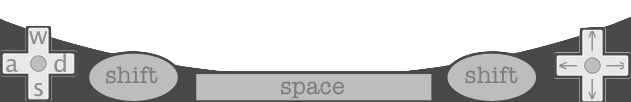
\includegraphics[width=0.6\textwidth]{videospiele/gamepad}
\end{center}
%
In der Signatur der Funktion entsprechen die
\lstinline{pad-event}-Werte den Tasten auf dem Pad:
%
\begin{lstlisting}
(world pad-event -> world)
\end{lstlisting}
%
\indexvariable{pad-event}
\begin{lstlisting}
(define pad-event
  (signature
    (enum "left" "right" "up" "down" "w" "s" "a" "d" " "
          "shift" "rshift")))
\end{lstlisting}
%
\begin{aufgabeinline}
  Erweitere den Aufruf von \lstinline{big-bang} so, dass man das Spiel
  auch mit dem Pad spielen kann!
\end{aufgabeinline}

\section*{Aufgaben}

\begin{aufgabe}
  Mache das Gürteltier-Spiel besser!
\end{aufgabe}

\begin{aufgabe}
  Schreibe ein Telespiel Deiner Wahl.
\end{aufgabe}

%%% Local Variables: 
%%% mode: latex
%%% TeX-master: "i1"
%%% End: 

